\subsection{Componenti delle Applicazioni}
Ogni applicazione Android è un archivio \textit{.apk} che contiene vari file in formato \textit{dex}. Ognuna di queste può svolgere innumerevoli funzioni, interagire con il sistema ed accedere a particolari tipi di dati condivisi. Di seguito andremo ad elencare ed analizzare i componenti principali che costituiscono ogni applicazione e che gli permettono di effettuare queste azioni.

\subsubsection{Activities}
L'\textit{Activity} è l'elemento principale di un'applicazione, rappresenta ogni schermata dell'app \cite{androides}, ne gestisce la logica di funzionamento e le interazioni con l'utente. Saranno presenti tante \textit{Activity} quante schermate. Queste non sono altro che un file Java.

È possibile definire l'aspetto di un'\textit{Activity} (i colori, gli elementi presenti, la loro posizione, ecc.) tramite un apposito file \textit{XML} (unico per ognuna) chiamato \textit{Layout} o tramite apposite funzioni e oggetti all'interno del codice Java.

\subsubsection{Intents}
Un \textit{Intent} è un meccanismo che serve per descrivere un'azione \cite{androides}: passare da un'Activity ad un'altra, scattare una foto, scegliere un'immagine dalla galleria, accedere alla posizione del GPS, ecc.
La creazione e l'utilizzo di un \textit{Intent} avvengono tramite apposite funzioni ed oggetti messi a disposizione dall'SDK.\\

\begin{lstlisting}[language=Java, caption=Esempio di codice Java per l'avvio di un'Activity tramite Intent]
    Intent intent = new Intent(
        this, 
        DisplayMessageActivity.class
    );
    startActivity(intent);
\end{lstlisting}

\subsubsection{Services}
In Android è possibile visualizzare ed interagire con una sola app alla volta, il che pone un grande limite nell'utilizzo. Per risolvere questo problema è possibile creare, per ogni applicazione, un \textit{Service} \cite{androides}: una specie di \textit{Unix Daemon}, privo di user interface, che rimane in esecuzione in background anche quando l'applicazione non è visibile o se ne sta utilizzando un'altra.

Un esempio è il lettore musicale che riesce a riprodurre file audio anche quando il telefono è bloccato o si utilizzano altre applicazioni.

\subsubsection{Content Providers}
Il \textit{Content Provider} è una parte di un'applicazione che si occupa di gestire un determinato set di dati e di regolarne gli accessi dalle altre app \cite{androides}.

Un esempio è il \textit{Content Provider} dell'app \textit{Contatti} che gestisce gli accessi, provenienti da altre applicazioni, ai dati salvati nella rubrica del telefono.\\

\begin{lstlisting}[language=Java, caption=Esempio di codice scritto in Java per una richiesta al Content Provider di User Dictionary]
    Cursor cursor = getContentResolver().query(
        UserDictionary.Words.CONTENT_URI,  
        projection,                        
        selectionClause,                   
        selectionArgs,                     
        sortOrder
    );                        
\end{lstlisting}

\begin{figure}[H]
  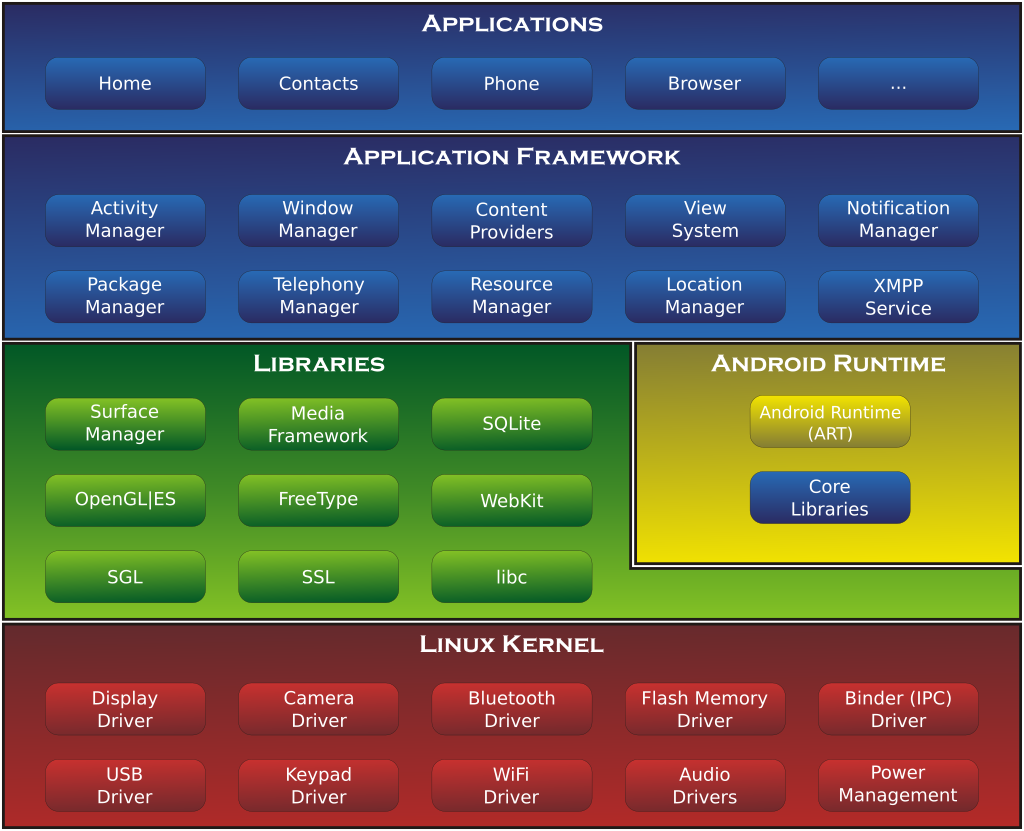
\includegraphics[scale=0.35]{android/imgs/android_new.png}
  \caption{Nuova architettura di Android}
  Questo è uno schema riassuntivo della nuova architettura di Android con la nuova ART.
\end{figure}
